% Created by tikzDevice version 0.8.1 on 2015-08-28 11:11:44
% !TEX encoding = UTF-8 Unicode
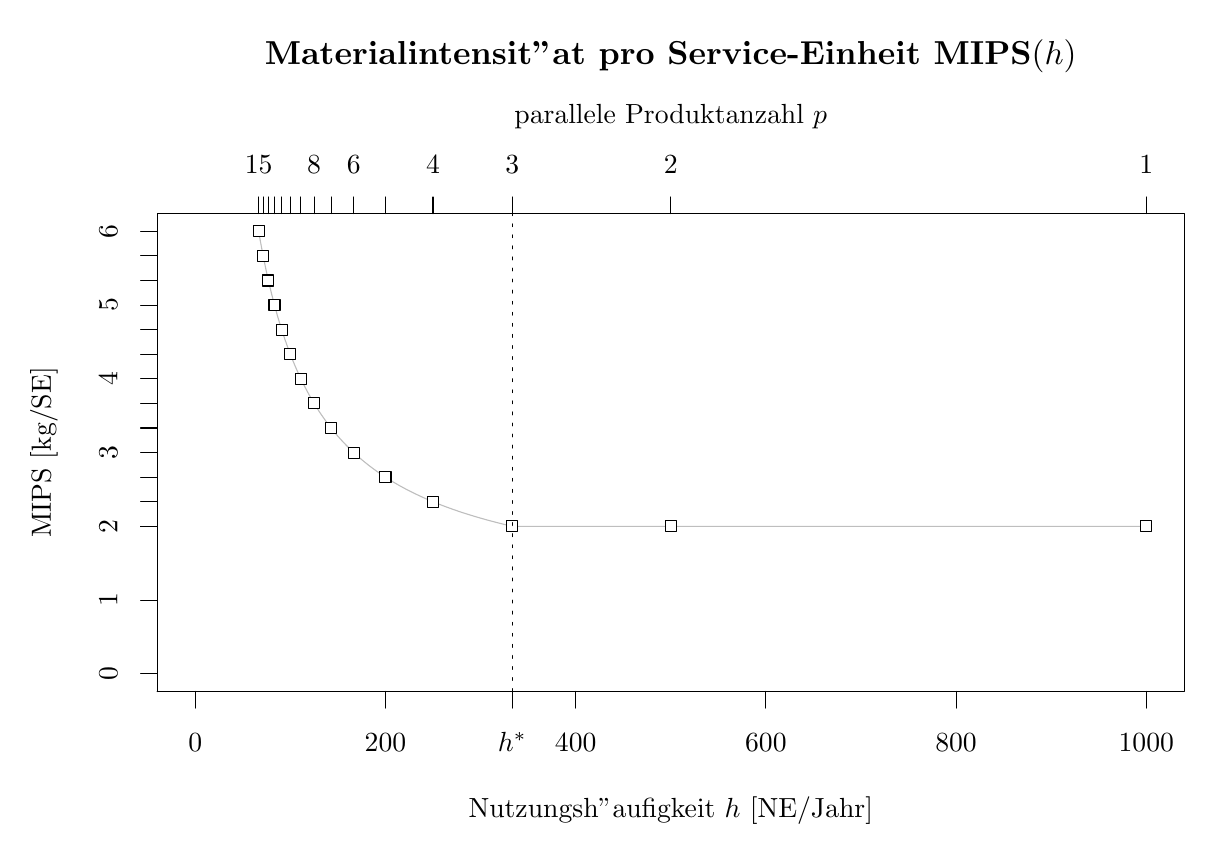
\begin{tikzpicture}[x=1pt,y=1pt]
\definecolor{fillColor}{RGB}{255,255,255}
\path[use as bounding box,fill=fillColor,fill opacity=0.00] (0,0) rectangle (419.17,289.08);
\begin{scope}
\path[clip] ( 46.80, 49.20) rectangle (417.97,221.88);
\definecolor{drawColor}{RGB}{190,190,190}

\path[draw=drawColor,line width= 0.4pt,line join=round,line cap=round] (404.22,108.89) --
	(381.63,108.89) --
	(361.83,108.89) --
	(344.33,108.89) --
	(328.75,108.89) --
	(314.79,108.89) --
	(302.21,108.89) --
	(290.82,108.89) --
	(280.45,108.89) --
	(270.98,108.89) --
	(262.29,108.89) --
	(254.29,108.89) --
	(246.90,108.89) --
	(240.05,108.89) --
	(233.69,108.89) --
	(227.76,108.89) --
	(222.23,108.89) --
	(217.05,108.89) --
	(212.19,108.89) --
	(207.62,108.89) --
	(203.33,108.89) --
	(199.27,108.89) --
	(195.44,108.89) --
	(191.82,108.89) --
	(188.38,108.89) --
	(185.12,108.89) --
	(182.02,108.89) --
	(179.08,108.89) --
	(176.27,108.89) --
	(173.59,109.25) --
	(171.03,109.87) --
	(168.59,110.50) --
	(166.25,111.12) --
	(164.01,111.75) --
	(161.87,112.37) --
	(159.81,113.00) --
	(157.83,113.62) --
	(155.93,114.25) --
	(154.10,114.87) --
	(152.35,115.50) --
	(150.65,116.12) --
	(149.02,116.75) --
	(147.45,117.37) --
	(145.93,118.00) --
	(144.46,118.62) --
	(143.04,119.25) --
	(141.67,119.87) --
	(140.35,120.50) --
	(139.07,121.12) --
	(137.82,121.75) --
	(136.62,122.37) --
	(135.45,123.00) --
	(134.32,123.62) --
	(133.23,124.25) --
	(132.16,124.87) --
	(131.13,125.50) --
	(130.12,126.12) --
	(129.14,126.75) --
	(128.19,127.37) --
	(127.27,128.00) --
	(126.37,128.62) --
	(125.50,129.25) --
	(124.64,129.87) --
	(123.81,130.50) --
	(123.00,131.12) --
	(122.22,131.75) --
	(121.45,132.37) --
	(120.70,133.00) --
	(119.97,133.62) --
	(119.25,134.25) --
	(118.55,134.87) --
	(117.87,135.50) --
	(117.21,136.12) --
	(116.56,136.75) --
	(115.92,137.37) --
	(115.30,138.00) --
	(114.70,138.62) --
	(114.10,139.24) --
	(113.52,139.87) --
	(112.95,140.49) --
	(112.40,141.12) --
	(111.85,141.74) --
	(111.32,142.37) --
	(110.80,142.99) --
	(110.29,143.62) --
	(109.78,144.24) --
	(109.29,144.87) --
	(108.81,145.49) --
	(108.34,146.12) --
	(107.88,146.74) --
	(107.42,147.37) --
	(106.98,147.99) --
	(106.54,148.62) --
	(106.11,149.24) --
	(105.69,149.87) --
	(105.28,150.49) --
	(104.87,151.12) --
	(104.47,151.74) --
	(104.08,152.37) --
	(103.70,152.99) --
	(103.32,153.62) --
	(102.95,154.24) --
	(102.58,154.87) --
	(102.22,155.49) --
	(101.87,156.12) --
	(101.52,156.74) --
	(101.18,157.37) --
	(100.85,157.99) --
	(100.52,158.62) --
	(100.19,159.24) --
	( 99.87,159.87) --
	( 99.56,160.49) --
	( 99.25,161.12) --
	( 98.95,161.74) --
	( 98.65,162.37) --
	( 98.35,162.99) --
	( 98.06,163.62) --
	( 97.78,164.24) --
	( 97.49,164.87) --
	( 97.22,165.49) --
	( 96.94,166.12) --
	( 96.68,166.74) --
	( 96.41,167.37) --
	( 96.15,167.99) --
	( 95.89,168.62) --
	( 95.64,169.24) --
	( 95.39,169.87) --
	( 95.14,170.49) --
	( 94.90,171.12) --
	( 94.66,171.74) --
	( 94.42,172.37) --
	( 94.19,172.99) --
	( 93.96,173.62) --
	( 93.73,174.24) --
	( 93.51,174.86) --
	( 93.29,175.49) --
	( 93.07,176.11) --
	( 92.85,176.74) --
	( 92.64,177.36) --
	( 92.43,177.99) --
	( 92.22,178.61) --
	( 92.02,179.24) --
	( 91.82,179.86) --
	( 91.62,180.49) --
	( 91.42,181.11) --
	( 91.23,181.74) --
	( 91.04,182.36) --
	( 90.85,182.99) --
	( 90.66,183.61) --
	( 90.48,184.24) --
	( 90.29,184.86) --
	( 90.11,185.49) --
	( 89.94,186.11) --
	( 89.76,186.74) --
	( 89.59,187.36) --
	( 89.42,187.99) --
	( 89.25,188.61) --
	( 89.08,189.24) --
	( 88.91,189.86) --
	( 88.75,190.49) --
	( 88.59,191.11) --
	( 88.43,191.74) --
	( 88.27,192.36) --
	( 88.11,192.99) --
	( 87.96,193.61) --
	( 87.81,194.24) --
	( 87.65,194.86) --
	( 87.50,195.49) --
	( 87.36,196.11) --
	( 87.21,196.74) --
	( 87.07,197.36) --
	( 86.92,197.99) --
	( 86.78,198.61) --
	( 86.64,199.24) --
	( 86.50,199.86) --
	( 86.36,200.49) --
	( 86.23,201.11) --
	( 86.09,201.74) --
	( 85.96,202.36) --
	( 85.83,202.99) --
	( 85.70,203.61) --
	( 85.57,204.24) --
	( 85.44,204.86) --
	( 85.32,205.49) --
	( 85.19,206.11) --
	( 85.07,206.74) --
	( 84.95,207.36) --
	( 84.82,207.99) --
	( 84.70,208.61) --
	( 84.59,209.24) --
	( 84.47,209.86) --
	( 84.35,210.49) --
	( 84.24,211.11) --
	( 84.12,211.73) --
	( 84.01,212.36) --
	( 83.90,212.98) --
	( 83.79,213.61) --
	( 83.68,214.23) --
	( 83.57,214.86) --
	( 83.46,215.48);
\definecolor{drawColor}{RGB}{0,0,0}
\definecolor{fillColor}{RGB}{255,255,255}

\path[draw=drawColor,line width= 0.4pt,line join=round,line cap=round,fill=fillColor] (402.23,106.90) rectangle (406.21,110.89);

\path[draw=drawColor,line width= 0.4pt,line join=round,line cap=round,fill=fillColor] (230.39,106.90) rectangle (234.38,110.89);

\path[draw=drawColor,line width= 0.4pt,line join=round,line cap=round,fill=fillColor] (173.11,106.90) rectangle (177.10,110.89);

\path[draw=drawColor,line width= 0.4pt,line join=round,line cap=round,fill=fillColor] (144.47,115.78) rectangle (148.46,119.77);

\path[draw=drawColor,line width= 0.4pt,line join=round,line cap=round,fill=fillColor] (127.29,124.66) rectangle (131.28,128.65);

\path[draw=drawColor,line width= 0.4pt,line join=round,line cap=round,fill=fillColor] (115.83,133.55) rectangle (119.82,137.53);

\path[draw=drawColor,line width= 0.4pt,line join=round,line cap=round,fill=fillColor] (107.65,142.43) rectangle (111.64,146.42);

\path[draw=drawColor,line width= 0.4pt,line join=round,line cap=round,fill=fillColor] (101.51,151.31) rectangle (105.50,155.30);

\path[draw=drawColor,line width= 0.4pt,line join=round,line cap=round,fill=fillColor] ( 96.74,160.19) rectangle (100.73,164.18);

\path[draw=drawColor,line width= 0.4pt,line join=round,line cap=round,fill=fillColor] ( 92.92,169.08) rectangle ( 96.91,173.06);

\path[draw=drawColor,line width= 0.4pt,line join=round,line cap=round,fill=fillColor] ( 89.80,177.96) rectangle ( 93.78,181.95);

\path[draw=drawColor,line width= 0.4pt,line join=round,line cap=round,fill=fillColor] ( 87.19,186.84) rectangle ( 91.18,190.83);

\path[draw=drawColor,line width= 0.4pt,line join=round,line cap=round,fill=fillColor] ( 84.99,195.73) rectangle ( 88.98,199.71);

\path[draw=drawColor,line width= 0.4pt,line join=round,line cap=round,fill=fillColor] ( 83.10,204.61) rectangle ( 87.09,208.60);

\path[draw=drawColor,line width= 0.4pt,line join=round,line cap=round,fill=fillColor] ( 81.46,213.49) rectangle ( 85.45,217.48);
\end{scope}
\begin{scope}
\path[clip] (  0.00,  0.00) rectangle (419.17,289.08);
\definecolor{drawColor}{RGB}{0,0,0}

\node[text=drawColor,anchor=base,inner sep=0pt, outer sep=0pt, scale=  1.00] at (232.38,  3.60) {Nutzungsh"aufigkeit $h$ [NE/Jahr]};

\node[text=drawColor,rotate= 90.00,anchor=base,inner sep=0pt, outer sep=0pt, scale=  1.00] at (  8.40,135.54) {MIPS [kg/SE]};
\end{scope}
\begin{scope}
\path[clip] ( 46.80, 49.20) rectangle (417.97,221.88);
\definecolor{drawColor}{RGB}{0,0,0}

\path[draw=drawColor,line width= 0.4pt,dash pattern=on 1pt off 3pt ,line join=round,line cap=round] (175.10, 49.20) -- (175.10,221.88);
\end{scope}
\begin{scope}
\path[clip] (  0.00,  0.00) rectangle (419.17,289.08);
\definecolor{drawColor}{RGB}{0,0,0}

\node[text=drawColor,anchor=base,inner sep=0pt, outer sep=0pt, scale=  1.20] at (232.38,275.88) {\bfseries Materialintensit"at pro Service-Einheit MIPS$(h)$};
\end{scope}
\begin{scope}
\path[clip] (  0.00,  0.00) rectangle (419.17,289.08);
\definecolor{drawColor}{RGB}{0,0,0}

\path[draw=drawColor,line width= 0.4pt,line join=round,line cap=round] ( 60.55, 49.20) -- (404.22, 49.20);

\path[draw=drawColor,line width= 0.4pt,line join=round,line cap=round] ( 60.55, 49.20) -- ( 60.55, 43.20);

\path[draw=drawColor,line width= 0.4pt,line join=round,line cap=round] (129.28, 49.20) -- (129.28, 43.20);

\path[draw=drawColor,line width= 0.4pt,line join=round,line cap=round] (175.10, 49.20) -- (175.10, 43.20);

\path[draw=drawColor,line width= 0.4pt,line join=round,line cap=round] (198.02, 49.20) -- (198.02, 43.20);

\path[draw=drawColor,line width= 0.4pt,line join=round,line cap=round] (266.75, 49.20) -- (266.75, 43.20);

\path[draw=drawColor,line width= 0.4pt,line join=round,line cap=round] (335.48, 49.20) -- (335.48, 43.20);

\path[draw=drawColor,line width= 0.4pt,line join=round,line cap=round] (404.22, 49.20) -- (404.22, 43.20);

\node[text=drawColor,anchor=base,inner sep=0pt, outer sep=0pt, scale=  1.00] at ( 60.55, 27.60) {0};

\node[text=drawColor,anchor=base,inner sep=0pt, outer sep=0pt, scale=  1.00] at (129.28, 27.60) {200};

\node[text=drawColor,anchor=base,inner sep=0pt, outer sep=0pt, scale=  1.00] at (175.10, 27.60) {$h^*$};

\node[text=drawColor,anchor=base,inner sep=0pt, outer sep=0pt, scale=  1.00] at (198.02, 27.60) {400};

\node[text=drawColor,anchor=base,inner sep=0pt, outer sep=0pt, scale=  1.00] at (266.75, 27.60) {600};

\node[text=drawColor,anchor=base,inner sep=0pt, outer sep=0pt, scale=  1.00] at (335.48, 27.60) {800};

\node[text=drawColor,anchor=base,inner sep=0pt, outer sep=0pt, scale=  1.00] at (404.22, 27.60) {1000};

\path[draw=drawColor,line width= 0.4pt,line join=round,line cap=round] ( 46.80, 55.60) -- ( 46.80,215.48);

\path[draw=drawColor,line width= 0.4pt,line join=round,line cap=round] ( 46.80, 55.60) -- ( 40.80, 55.60);

\path[draw=drawColor,line width= 0.4pt,line join=round,line cap=round] ( 46.80, 82.24) -- ( 40.80, 82.24);

\path[draw=drawColor,line width= 0.4pt,line join=round,line cap=round] ( 46.80,108.89) -- ( 40.80,108.89);

\path[draw=drawColor,line width= 0.4pt,line join=round,line cap=round] ( 46.80,108.89) -- ( 40.80,108.89);

\path[draw=drawColor,line width= 0.4pt,line join=round,line cap=round] ( 46.80,108.89) -- ( 40.80,108.89);

\path[draw=drawColor,line width= 0.4pt,line join=round,line cap=round] ( 46.80,117.77) -- ( 40.80,117.77);

\path[draw=drawColor,line width= 0.4pt,line join=round,line cap=round] ( 46.80,126.66) -- ( 40.80,126.66);

\path[draw=drawColor,line width= 0.4pt,line join=round,line cap=round] ( 46.80,135.54) -- ( 40.80,135.54);

\path[draw=drawColor,line width= 0.4pt,line join=round,line cap=round] ( 46.80,144.42) -- ( 40.80,144.42);

\path[draw=drawColor,line width= 0.4pt,line join=round,line cap=round] ( 46.80,153.31) -- ( 40.80,153.31);

\path[draw=drawColor,line width= 0.4pt,line join=round,line cap=round] ( 46.80,162.19) -- ( 40.80,162.19);

\path[draw=drawColor,line width= 0.4pt,line join=round,line cap=round] ( 46.80,171.07) -- ( 40.80,171.07);

\path[draw=drawColor,line width= 0.4pt,line join=round,line cap=round] ( 46.80,179.95) -- ( 40.80,179.95);

\path[draw=drawColor,line width= 0.4pt,line join=round,line cap=round] ( 46.80,188.84) -- ( 40.80,188.84);

\path[draw=drawColor,line width= 0.4pt,line join=round,line cap=round] ( 46.80,197.72) -- ( 40.80,197.72);

\path[draw=drawColor,line width= 0.4pt,line join=round,line cap=round] ( 46.80,206.60) -- ( 40.80,206.60);

\path[draw=drawColor,line width= 0.4pt,line join=round,line cap=round] ( 46.80,215.48) -- ( 40.80,215.48);

\node[text=drawColor,rotate= 90.00,anchor=base,inner sep=0pt, outer sep=0pt, scale=  1.00] at ( 32.40, 55.60) {0};

\node[text=drawColor,rotate= 90.00,anchor=base,inner sep=0pt, outer sep=0pt, scale=  1.00] at ( 32.40, 82.24) {1};

\node[text=drawColor,rotate= 90.00,anchor=base,inner sep=0pt, outer sep=0pt, scale=  1.00] at ( 32.40,108.89) {2};

\node[text=drawColor,rotate= 90.00,anchor=base,inner sep=0pt, outer sep=0pt, scale=  1.00] at ( 32.40,135.54) {3};

\node[text=drawColor,rotate= 90.00,anchor=base,inner sep=0pt, outer sep=0pt, scale=  1.00] at ( 32.40,162.19) {4};

\node[text=drawColor,rotate= 90.00,anchor=base,inner sep=0pt, outer sep=0pt, scale=  1.00] at ( 32.40,188.84) {5};

\node[text=drawColor,rotate= 90.00,anchor=base,inner sep=0pt, outer sep=0pt, scale=  1.00] at ( 32.40,215.48) {6};

\path[draw=drawColor,line width= 0.4pt,line join=round,line cap=round] ( 83.46,221.88) -- (404.22,221.88);

\path[draw=drawColor,line width= 0.4pt,line join=round,line cap=round] ( 83.46,221.88) -- ( 83.46,227.88);

\path[draw=drawColor,line width= 0.4pt,line join=round,line cap=round] ( 85.09,221.88) -- ( 85.09,227.88);

\path[draw=drawColor,line width= 0.4pt,line join=round,line cap=round] ( 86.98,221.88) -- ( 86.98,227.88);

\path[draw=drawColor,line width= 0.4pt,line join=round,line cap=round] ( 89.19,221.88) -- ( 89.19,227.88);

\path[draw=drawColor,line width= 0.4pt,line join=round,line cap=round] ( 91.79,221.88) -- ( 91.79,227.88);

\path[draw=drawColor,line width= 0.4pt,line join=round,line cap=round] ( 94.91,221.88) -- ( 94.91,227.88);

\path[draw=drawColor,line width= 0.4pt,line join=round,line cap=round] ( 98.73,221.88) -- ( 98.73,227.88);

\path[draw=drawColor,line width= 0.4pt,line join=round,line cap=round] (103.51,221.88) -- (103.51,227.88);

\path[draw=drawColor,line width= 0.4pt,line join=round,line cap=round] (109.64,221.88) -- (109.64,227.88);

\path[draw=drawColor,line width= 0.4pt,line join=round,line cap=round] (117.83,221.88) -- (117.83,227.88);

\path[draw=drawColor,line width= 0.4pt,line join=round,line cap=round] (129.28,221.88) -- (129.28,227.88);

\path[draw=drawColor,line width= 0.4pt,line join=round,line cap=round] (146.46,221.88) -- (146.46,227.88);

\path[draw=drawColor,line width= 0.4pt,line join=round,line cap=round] (175.10,221.88) -- (175.10,227.88);

\path[draw=drawColor,line width= 0.4pt,line join=round,line cap=round] (232.38,221.88) -- (232.38,227.88);

\path[draw=drawColor,line width= 0.4pt,line join=round,line cap=round] (404.22,221.88) -- (404.22,227.88);

\node[text=drawColor,anchor=base,inner sep=0pt, outer sep=0pt, scale=  1.00] at ( 83.46,236.28) {15};

\node[text=drawColor,anchor=base,inner sep=0pt, outer sep=0pt, scale=  1.00] at (103.51,236.28) {8};

\node[text=drawColor,anchor=base,inner sep=0pt, outer sep=0pt, scale=  1.00] at (117.83,236.28) {6};

\node[text=drawColor,anchor=base,inner sep=0pt, outer sep=0pt, scale=  1.00] at (146.46,236.28) {4};

\node[text=drawColor,anchor=base,inner sep=0pt, outer sep=0pt, scale=  1.00] at (175.10,236.28) {3};

\node[text=drawColor,anchor=base,inner sep=0pt, outer sep=0pt, scale=  1.00] at (232.38,236.28) {2};

\node[text=drawColor,anchor=base,inner sep=0pt, outer sep=0pt, scale=  1.00] at (404.22,236.28) {1};

\path[draw=drawColor,line width= 0.4pt,line join=round,line cap=round] ( 46.80, 49.20) --
	(417.97, 49.20) --
	(417.97,221.88) --
	( 46.80,221.88) --
	( 46.80, 49.20);

\node[text=drawColor,anchor=base,inner sep=0pt, outer sep=0pt, scale=  1.00] at (232.38,254.28) {parallele Produktanzahl $p$};
\end{scope}
\end{tikzpicture}
